\documentclass[12pt,a4paper]{exam}
\usepackage[utf8]{inputenc}
\usepackage[catalan]{babel}
\usepackage{graphicx}
\usepackage{geometry}
\usepackage{fancyhdr}
\usepackage{tabularx}
\usepackage{lastpage}
\usepackage{amsmath}
\usepackage{amsfonts}

% ACTIVAR SOLUCIONS
\printanswers 
\renewcommand{\solutiontitle}{\noindent\textbf{Solució:}\enspace}

% 1. MARGES I CAPÇALERA
\geometry{top=4cm, bottom=3.5cm, left=2cm, right=2cm, headheight=2.5cm}

\pagestyle{fancy}
\fancyhf{}
\fancyhead[L]{
\includegraphics[height=1.8cm]{Logo_Departament.png}} 
\fancyhead[R]{
\includegraphics[height=1.8cm]{Logo_Institut.png}}
\renewcommand{\headrulewidth}{0.4pt}

% 2. PEU DE PÀGINA
\fancyfoot[C]{
    \begin{tabularx}{\textwidth}{|>{\centering\arraybackslash}X|>{\centering\arraybackslash}X|>{\centering\arraybackslash}X|}
        \hline
        Institut Nou de Vic & Prova d'avaluació: Funcions & Pàgina \thepage\ de \pageref{LastPage} \\ \hline
    \end{tabularx}
}

\begin{document}

% 3. TAULA DE DADES
\noindent
\begingroup
\renewcommand{\arraystretch}{2}
\begin{tabularx}{\textwidth}{|X|X|c|}
    \hline
    \multicolumn{2}{|l|}{Cognoms i Nom:} & Qualificació \\ \hline
    Data: & Curs: 1r Batxillerat CCSS &  \\ \cline{1-2}
    Matèria: Matemàtiques aplicades & Prova: Examen de Funcions & \smash{\lower.5\arraystretch\hbox{}} \\ \hline
\end{tabularx}
\endgroup

\vspace{0.6cm}

\begin{questions}

% EXERCICI 1
\question (1 punt) Troba el domini de les següents funcions:
\begin{parts}
    \part $f(x) = x^2 - 5x + 6$
    \part $g(x) = \dfrac{x + 1}{x^2 - 4}$
    \part $h(x) = \sqrt{x - 5}$
    \part $i(x) = \sqrt[3]{x-4}$
\end{parts}

\begin{solution}
\begin{itemize}
    \item \textbf{a)} Funció polinòmica: $D(f) = \mathbb{R}$ o $(-\infty, +\infty)$.
    \item \textbf{b)} Funció racional. Calculem quan el denominador és zero: $x^2 - 4 = 0 \Rightarrow x^2 = 4 \Rightarrow x = \pm 2$. Per tant, $D(g) = \mathbb{R} \setminus \{-2, 2\}$.
    \item \textbf{c)} Funció radical d'índex parell. L'interior ha de ser $\geq 0$: $x - 5 \geq 0 \Rightarrow x \geq 5$. Per tant, $D(h) = [5, +\infty)$.
    \item \textbf{d)} Funció radical d'índex senar. Com que l'interior és un polinomi, el domini són tots els Reals: $D(i) = \mathbb{R}$.
\end{itemize}
\end{solution}

% EXERCICI 2
\question (1 punt) Donades les funcions $f(x) = 2x + 3$ i $g(x) = x^2 + 4$, calcula l'expressió algebraica i indica el domini de:
\begin{parts}
    \part $(f - g)(x)$
    \part $(f \cdot g)(x)$
    \part $\left(\dfrac{f}{g}\right)(x)$ 
    \part $(g \circ f)(x)$ 
\end{parts}

\begin{solution}
\begin{itemize}
    \item \textbf{a)} $(2x+3) - (x^2+4) = -x^2 + 2x - 1$. Domini: $\mathbb{R}$.
    \item \textbf{b)} $(2x+3) \cdot (x^2+4) = 2x^3 + 8x + 3x^2 + 12 = 2x^3 + 3x^2 + 8x + 12$. Domini: $\mathbb{R}$.
    \item \textbf{c)} $\frac{2x+3}{x^2+4}$. Com que $x^2+4$ mai és zero (sempre és positiu), el domini és $\mathbb{R}$.
    \item \textbf{d)} $g(f(x)) = (2x+3)^2 + 4 = 4x^2 + 12x + 9 + 4 = 4x^2 + 12x + 13$. Domini: $\mathbb{R}$.
\end{itemize}
\end{solution}

% EXERCICI 3
\question (1 punt) Donada la funció $f(x) = \dfrac{4}{x + 1}$:
\begin{parts}
    \part Troba la seva funció inversa $f^{-1}(x)$.
    \part Indica quin és el recorregut de la funció original $f(x)$.
\end{parts}

\begin{solution}
\begin{itemize}
    \item \textbf{a)} Fem $y = \frac{4}{x+1}$. Aillem la $x$: $x+1 = \frac{4}{y} \Rightarrow x = \frac{4}{y} - 1$. Intercanviem variables: $f^{-1}(x) = \frac{4}{x} - 1 = \frac{4-x}{x}$.
    \item \textbf{b)} El recorregut de $f$ és el domini de $f^{-1}$. Com que a $f^{-1}$ la $x$ no pot ser $0$, el Recorregut de $f(x) = \mathbb{R} \setminus \{0\}$.
\end{itemize}
\end{solution}

% EXERCICI 4
\question (1 punt) Relaciona les expressions algebraiques següents amb les funcions de la representació gràfica tot \textbf{justificant la resposta}

\begin{minipage}[t]{0.45\textwidth}
    \begin{parts}
        \part $\mathbf{f_5}(x)=x^2-4x+3$
        \part $\mathbf{f_4}(x)= -3x - 2$
        \part $\mathbf{f_3}(x) = 2x - 2$
        \part $\mathbf{f_1}(x)= x^2 - 4x$
        \part $\mathbf{f_2}(x)= x - 2$
    \end{parts}
\end{minipage}
\hfill
\begin{minipage}[t]{0.3\textwidth}
    \centering
    \vspace{0pt}
    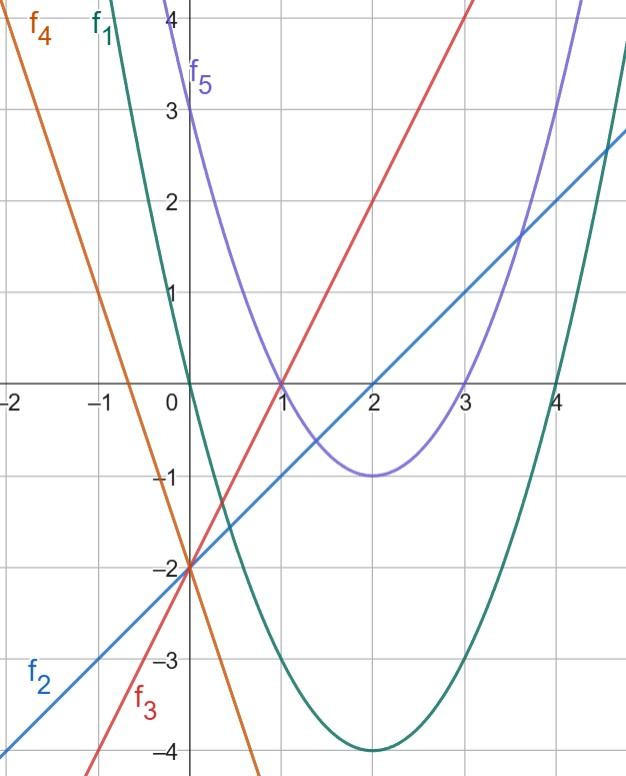
\includegraphics[width=\textwidth]{funcions.jpg} 
\end{minipage}

\begin{solution}
\begin{itemize}
    \item \textbf{$f_5$} és la paràbola morada que talla l'eix Y a 3 i té arrels a 1 i 3.
    \item \textbf{$f_4$} és la recta taronja amb pendent negatiu que talla Y a -2.
    \item \textbf{$f_3$} és la recta vermella amb pendent positiu fort ($m=2$) que talla Y a -2.
    \item \textbf{$f_1$} és la paràbola negra que passa per l'origen (talla Y a 0).
    \item \textbf{$f_2$} és la recta blava amb pendent positiu suau ($m=1$) que talla Y a -2.
\end{itemize}
\end{solution}


% EXERCICI 5
\question (1 punt) Troba el punt d'intersecció (punt on es creuen) les gràfiques de les funcions $f(x) = 2x + 1$ i $g(x) = -x + 4$.

\begin{solution}
Igualem les funcions: $2x + 1 = -x + 4 \Rightarrow 3x = 3 \Rightarrow x = 1$. \\
Trobem la coordenada $y$: $y = 2(1) + 1 = 3$. \\
El punt d'intersecció és \textbf{P(1, 3)}.
\end{solution}

\question (1 punt) Representa gràficament la funció quadràtica $f(x) = x^2 - 6x + 5$. Calcula:
\begin{parts}
    \part L'orientació i les coordenades del vèrtex.
    \part Els punts de tall amb els eixos horitzontal i vertical.
    \part Dibuixa la gràfica.
\end{parts}

% Dins de la solució de l'exercici 6:
\begin{solution}
\begin{itemize}
    \item \textbf{a)} Orientació: cap amunt ($a=1$). Vèrtex: $x_v = \frac{-(-6)}{2} = 3$; $y_v = 3^2 - 6(3) + 5 = -4$. \textbf{V(3, -4)}.
    \item \textbf{b)} Tall Y: $(0, 5)$. Tall X: $x^2 - 6x + 5 = 0 \Rightarrow (x-1)(x-5)=0$. Punts: \textbf{(1, 0)} i \textbf{(5, 0)}.
    \item \textbf{c)} \textbf{Taula de valors:}
\end{itemize}

\begin{center}
\begin{tabular}{|c|c|c|c|c|c|c|c|}
    \hline
    $x$ & 0 & 1 & 2 & \textbf{3} & 4 & 5 & 6 \\ \hline
    $f(x)$ & 5 & 0 & -3 & \textbf{-4} & -3 & 0 & 5 \\ \hline
\end{tabular}
\end{center}
\end{solution}
% EXERCICI 7
\question (1 punt) Troba l'expressió algebraica de la funció quadràtica $f(x) = ax^2 + bx + c$ que passa pels punts $A(0, 2)$, $B(1, 3)$ i $C(-1, 5)$.

\begin{solution}
\begin{enumerate}
    \item Del punt A(0, 2) sabem que $c = 2$.
    \item Del punt B(1, 3): $a(1)^2 + b(1) + 2 = 3 \Rightarrow a + b = 1$.
    \item Del punt C(-1, 5): $a(-1)^2 + b(-1) + 2 = 5 \Rightarrow a - b = 3$.
    \item Sumant les equacions: $2a = 4 \Rightarrow a = 2$. Llavors $b = 1 - 2 = -1$.
    \item L'expressió és \textbf{$f(x) = 2x^2 - x + 2$}.
\end{enumerate}
\end{solution}

% EXERCICI 8
\question (1 punt) Observa la gràfica de la funció definida a trossos (adjunta) i respon:
\begin{parts}
    \part Indica el domini i el recorregut de la funció.
    \part Quins són els punts de tall amb els eixos?
    \part Determina els intervals de creixement i decreixement.
    \part Indica els màxims i mínims (especifica si sòn relatius o absoluts).
    \part És una funció contínua? Si no ho és, indica on no ho és.
\end{parts}

\begin{solution}
Basant-nos en la gràfica `CaracteristiquesFuncions.png`:
\begin{itemize}
    \item \textbf{a)} Domini: $\mathbb{R}$. Recorregut: $(-\infty, 4]$.
    \item \textbf{b)} Tall Y: $(0, 0)$. Tall X: $(-5, 0)$ i $(0, 0)$.
    \item \textbf{c)} Creix: $(-\infty, -3) \cup (-1, 2) \cup (3, +\infty)$. Decreix: $(-3, -1) \cup (2, 3)$.
    \item \textbf{d)} Màxim Absolut a $(-3, 4)$. Màxim Relatiu a $(2, 2)$. Mínim Relatiu a $(3, 1)$ i $(-1, -1)$.
    \item \textbf{e)} No és contínua. Té un salt finit (discontinuïtat de salt) a \textbf{$x = -1$}.
\end{itemize}
\end{solution}

% ESPAI PER A LA IMATGE DE GEOGEBRA
\begin{center}
    \fbox{\begin{minipage}{0.8\textwidth} \centering  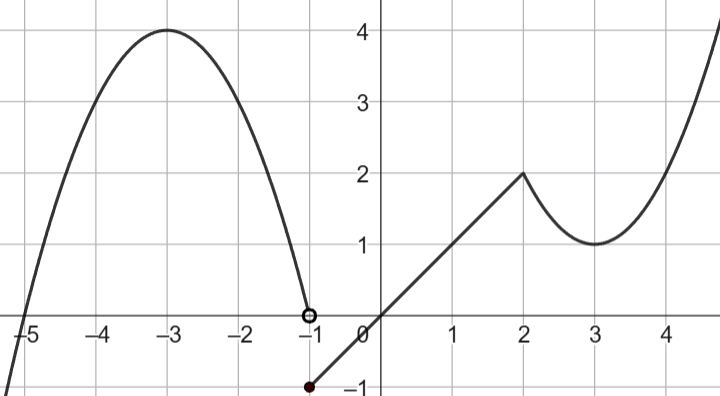
\includegraphics[width=\textwidth]{CaracteristiquesFuncions.png} 
    \end{minipage}}
\end{center}

\vspace{0.3cm}

% EXERCICI 9
\question (1 punt) Unes vambes de col·leccionista valien $120$ € en sortir al mercat (mes 0). Al cap de $3$ mesos, el seu valor és de $170$ €. $3$ mesos després tenen un valor de $225 €$. Suposant un creixement lineal, quin era el valor de les vambes després de 4 mesos i mig?

\begin{solution}
\begin{enumerate}
    \item Punts de l'interval corresponent ($x=4.5$ està entre $3$ i $6$): $A(3, 170)$ i $B(6, 225)$.
    \item Pendent del segment: $m = \frac{225 - 170}{6 - 3} = \frac{55}{3} \approx 18.33$ €/mes.
    \item Equació de la recta en aquest tram: $y - 170 = \frac{55}{3}(x - 3)$.
    \item Per $x = 4.5$: 
    $y = \frac{55}{3}(4.5 - 3) + 170 = \frac{55}{3}(1.5) + 170 = 55 \cdot 0.5 + 170 = 27.5 + 170 = \textbf{197.5 €}$.
\end{enumerate}
\end{solution}

% EXERCICI 10
\question (1 punt) Una empresa d'impressió de samarretes cobra 20 € de despeses fixes de disseny i 8 € per cada samarreta impresa.
\begin{parts}
    \part Escriu l'expressió algebraica de la funció cost $f(x)$ segons el nombre de samarretes $x$.
    \part Què signifiquen el pendent i l'ordenada a l'origen en aquest context?
    \part Calcula el cost total de fer 15 samarretes.
    \part Si hem pagat 140 €, quantes samarretes hem comprat?
\end{parts}

\begin{solution}
\begin{itemize}
    \item \textbf{a)} $f(x) = 8x + 20$.
    \item \textbf{b)} Pendent ($m=8$): preu per cada samarreta. Ordenada ($n=20$): cost fix inicial de disseny.
    \item \textbf{c)} $f(15) = 8(15) + 20 = 120 + 20 = \textbf{140 €}$.
    \item \textbf{d)} $140 = 8x + 20 \Rightarrow 120 = 8x \Rightarrow x = \textbf{15 samarretes}$.
\end{itemize}
\end{solution}


\end{questions}
\end{document}